
%(BEGIN_QUESTION)
% Copyright 2011, Tony R. Kuphaldt, released under the Creative Commons Attribution License (v 1.0)
% This means you may do almost anything with this work of mine, so long as you give me proper credit

Determine whether this controller implements a {\it proportional-only}, {\it integral-only}, or {\it proportional plus integral} algorithm.

$$\includegraphics[width=15.5cm]{i01901x01.eps}$$

\hbox{ \vrule
\vbox{ \hrule \vskip 3pt
\hbox{ \hskip 3pt
\vbox{ \hsize=5in \raggedright

\noindent
\underbar{\bf Pseudocode listing}

{\tt Declare Pin0 as an analog input (scale 0 to 5 volts = 0 to 1023)}

{\tt Declare Pin1 as an analog output (scale 0 to 5 volts = 0 to 1023)}

{\tt Declare SP as a variable, initially set to a value of 614}

{\tt Declare GAIN as a variable, initially set to a value of 1.0}

{\tt Declare K as a variable, initially set to a value of 1.0}

{\tt Declare X as a variable, initially set to a value of 614}

{\tt Declare ERROR as a variable}

{\tt Declare T as a variable}

{\tt Declare LAST\_T as a variable}

\vskip 10pt

{\tt LOOP}

\hskip 10pt {\tt SET ERROR = Pin0 - SP}

\hskip 10pt {\tt SET X = X + (ERROR * K * (T - LAST\_T))}

\hskip 10pt {\tt SET Pin1 = (GAIN * ERROR) + X}

\hskip 10pt {\tt SET LAST\_T = T}

\hskip 10pt {\tt SET T = system\_clock\_time}

{\tt ENDLOOP}
}
\hskip 3pt}%
\vskip 5pt \hrule}%
\vrule}

\vskip 10pt

Now, assuming you cannot change any part of the programming code -- but you are allowed to add any electronic components you wish to the circuit -- determine a way to add derivative action to the existing actions exhibited by this controller. 

\underbar{file i01901}
%(END_QUESTION)





%(BEGIN_ANSWER)

I recommend 5 points for the correct actions, and 5 points for a workable solution:

\vskip 10pt

The action as programmed is {\bf proportional plus integral}.  

\vskip 10pt

In order to add derivative action, you must incorporate a differentiator circuit in such a way that it {\it adds} to the microcontroller's output.  Here is one possible solution:

$$\includegraphics[width=15.5cm]{i01901x02.eps}$$

An answer consisting of an active differentiator circuit simply connected to the microcontroller's output pin does not count, because this would prevent proportional and integral actions from making it to the final $V_{out}$.

$$\includegraphics[width=15.5cm]{i01901x03.eps}$$

%(END_ANSWER)





%(BEGIN_NOTES)

{\bf This question is intended for exams only and not worksheets!}.

%(END_NOTES)


